\setstretch{1.5}
\chapter{Dynamic Modeling of the Plasma Generation Process}


\tab In the traditional control of plasma etch tools very few process characteristics are regulated in real time. While the quality of the etch is determined by the etch characteristics presented in Section 1.1.2, real-time in situ measurement of these characteristics is difficult (if not impossible). Therefore, these etch characteristics cannot be used to control the etching process; instead, process recipes are often specified only in terms of equipment setpoints. These setpoints affect the etch characteristics only indirectly through the plasma properties. In some sense, the process engineer is handicapped in that there is only access to equipment inputs, rather than plasma parameters. As the plasma characteristics strongly influence the etch properties, controlling the plasma generation process has the potential for improving the quality of the etch. This forms the basis for the control strategies pursued
in this research.

\setstretch{1}
\section{Control-Oriented Decomposition and Control Strategy.}

\setstretch{1.5}

\tab We begin by “conceptually” decomposing the etch into two separate, but interacting, processes; the plasma generation process (PGP) and the wafer etch process (WEP). This decomposition is shown graphically in Figure 3.1. These sequential processes separate the generation of the important chemical and physical species from the action of etching the surface of the wafer. The inputs to the PGP are the various equipment settings (\textit{e.g.} throttle position, gas composition and flow rates, and applied power); the outputs are the key plasma parameters that are responsible for etching (\textit{e.g.} $V_{bias}$, pressure, ion flux,and the concentration of neutral radicals and polymer precursors\footnote{It is actually the flux of these species to the wafer surface that affects the etching process. However, as was shown in Section 1.2.2, the flux of each species is closely related to its concentration in the bulk plasma.}). The WEP is driven by these plasma parameters and has as outputs the characteristics crucial to etch performance. This decomposition actually represents a physical separation: the PGP represents the bulk plasma, the W EP represents the wafer surface phenomena, and the interface between them is the sheath. It is important to note that there does exist a certain amount of feedback coupling from the wafer surface to the plasma (see, for example, the loading effect in Section 4.2.1). The wafer itself is therefore a disturbance to the plasma generation process.

It is desirable to control the five plasma characteristics shown in Figure 3.1. While there are well established methods of measuring both $V_{bias}$ and pressure, custom sensors are necessary for the measurement of the other characteristics. Unfortunately, of these characteristics, we are presently only able to estimate the concentration of the fluorine radicals. Separate research projects are underway to measure ion current (flux) through rf electrical measurements and polymer precursors using optical emission spectroscopy. For the rest of this dissertation, control of plasma parameters will be limited to $V_{bias}$ pressure, and fluorine concentration ([F]).


The above decomposition of the RIE leads to our control structure. The key idea is to regulate the inputs to the WEP by precisely controlling the outputs of the PGP. This is accomplished by designing a real-time controller for the PG P as shown in Figure 3.2.

\setstretch{1}
\begin{figure}[H]
	\centering
	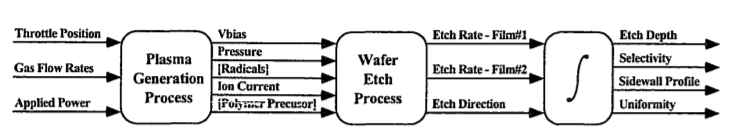
\includegraphics[scale = .7]{Figure 3.1}
	\bf\caption{ Conceptual decomposition of the RIE process.}
	\label{fig:3.1}
\end{figure}

\setstretch{1.5}

\noindent Future research is expected to include the development of a controller around the WEP and a supervisory level controller. The W EP controller will translate desired etch characteristics into setpoints for the PGP control system. The supervisory controller will perform the highlevel cell control functions that include on-line monitoring, diagnostics, and failure recovery as well as post-process analysis of the data for the purposes of sequential optimization, quality control, and so forth. At present, only the PGP controller has been implemented.

There are many merits to this approach:

\begin{itemize}
	\item W ith existing sensor technology, it is very difficult to measure the key wafer etch parameters (selectivity, anisotropy, etc.) in real time during the etch process. (Some of these can be measured in near-real-time.) Therefore, for real-time feedback control,an indirect strategy is necessary.
	
	\item
	Modeling of the etch characteristics is the most difficult part of the problem. With this controller structure, the modeling task may become more tractable. The model for the PGP can be developed first, leading to the development of the real-time plasma controller. Then the modeling task for the WEP would involve relating the effects of the key plasma parameters on the etch performance, which is much more direct than trying to build a single model from the equipment inputs to the etch characteristics.
	
	
	\item The switch from specifying the process recipes in terms of [throttle position, flow rates,
	
	\begin{figure}[H]
		\centering
		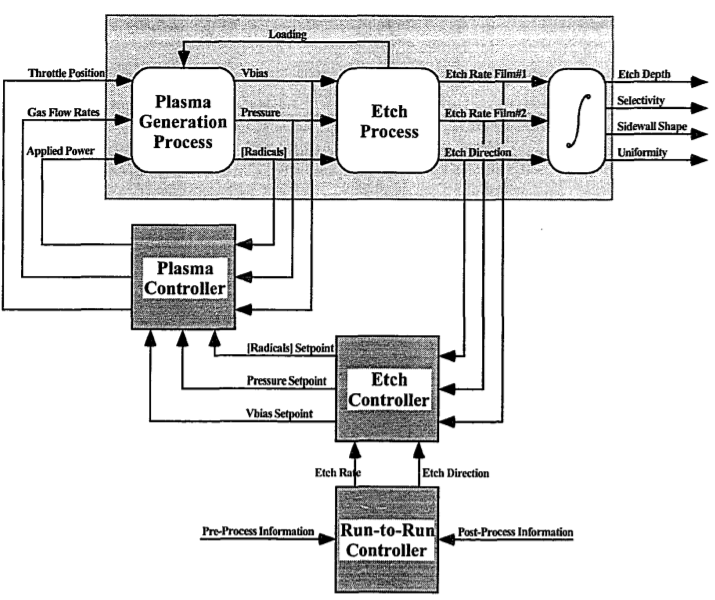
\includegraphics[scale = .7]{Figure 3.2}
		\bf\caption{ Feedback control strategy for th e reactive ion etching process.}
		\label{fig:3.2}
	\end{figure}
	
	power] to [$V_{bias}$, pressure, fluorine concentration] is a significant change of viewpoint. As was seen in Section 1.2.2, these new setpoints are, in many ways, more directly
	connected to the overall etch performance; tightly regulating them should eliminate much of the variance seen in plasma systems. Using plasma characteristics as setpoints may also facilitate the exchange of process recipes between different systems.
	
\end{itemize}

\section{System Identification of the Plasma Generation Process}

\tab The PGP controller is based upon a dynamic model of the plasma generation process. While the PGP is highly nonlinear, a linear model was desired to allow the use of linear control design techniques. Thus, instead of modeling the process dynamics over a wide range of operating conditions, a model was developed that captured the process dynamics in a small region around a give operating point. Two major factors in choosing this operating point were that the etching was in an RIE regime (both chemical and physical) and that the actuators have good authority over the plasma properties. Roughly, the AME-8300 is in an RIE regime for pressures below 50 mTorr and power above 500W.

The nonlinear nature of the throttle valve made it difficult to determine \textit{a priori} its region of highest authority. In the next section, the procedure for determining the throttle settings at which the throttle valve has maximum authority as an actuator is described. This throttle position, along with the $\text{CF}_{4}$ flow rate required to make pressure approximately 20 mTorr and a power of 1000W, defined the operating point used for the modeling of the plasma generation process.

\subsection{Conductance Through the Throttle Valve}

\tab The throttle valve is nonlinear in nature and has different levels of authority at various throttle positions and chamber pressures. Therefore, a set of experiments was devised to find an operating region where the valve was most effective in influencing the pressure.

First, the chamber was sealed from the pump stack by closing the turbo gate valve. The chamber was then filled with $\text{CF}_{4}$ to approximately 85 mTorr, after which the $\text{CF}_{4}$ flow was shut off. The throttle was then set to the desired position; experiments were run at throttle positions

\begin{align}
	\theta = [2.5,5.0,7.5,... , 22.5,25.0] (\% \text{Open}).
\end{align}

\noindent Finally, the turbo gate valve was opened and the pressure was monitored as the chamber was pumped out. A plot of pressure vs. time for the throttle setting $\theta$=12.5 \% Open is shown in Figure 3.3.

Flow can be expressed in terms of a volume per unit time

\setstretch{1}
\begin{align}
	\frac{dV}{dt} = \frac{dn}{dt}\frac{RT_{STP}}{P_{STP}},
\end{align}

\setstretch{1.5}
\noindent where $\frac{dn}{dt}$ is the change in moles of $\text{CF}_{4}$ per unit time, R is the universal gas constant, $T_{stp}$ is standard temperature (298 ° K ) and $P_{stp}$ is standard pressure (760 Torr). The slope of the pressure curve from Figure 3.3 (shown in Figure 3.4 is related to $\frac{dn}{dt}$ by

\setstretch{1}
\begin{align}
	\frac{dn}{dt} = \frac{dP}{dt}\frac{V_{cham}}{RT_{STP}},
\end{align}

\setstretch{1.5}
\noindent where $V_{cham}$ is the volume of the chamber. Thus, the flow through the throttle valve can be found from


\setstretch{1}
\begin{align}
	\frac{dV}{dt} = \frac{dP}{dt}\frac{V_{cham}}{RT_{STP}}.
\end{align}


\begin{figure}[H]
	\centering
	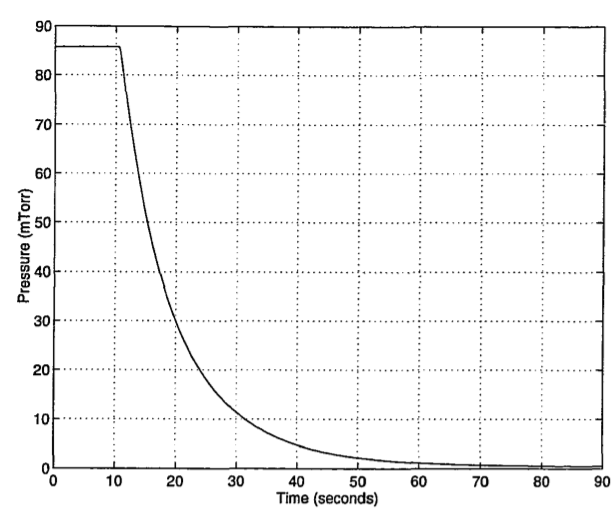
\includegraphics[scale = .6]{Figure 3.3}
	\bf\caption{ Pressure response during conductance experiment.}
	\label{fig:3.3}
\end{figure}

\begin{figure}[H]
	\centering
	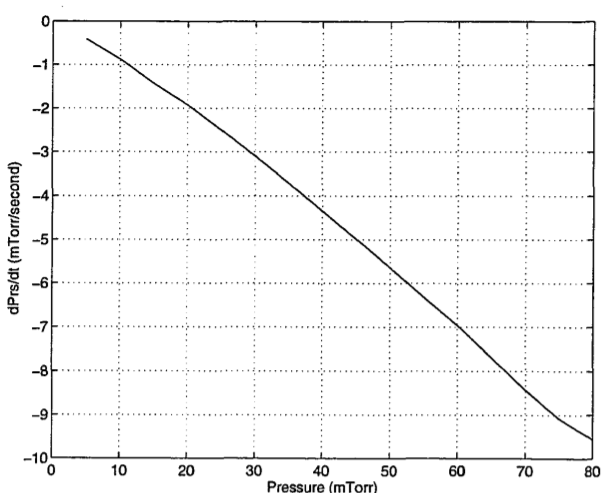
\includegraphics[scale = .6]{Figure 3.4}
	\bf\caption{ dPrs/dt vs. pressure during conductance experiment.}
	\label{fig:3.4}
\end{figure}

\begin{figure}[H]
	\centering
	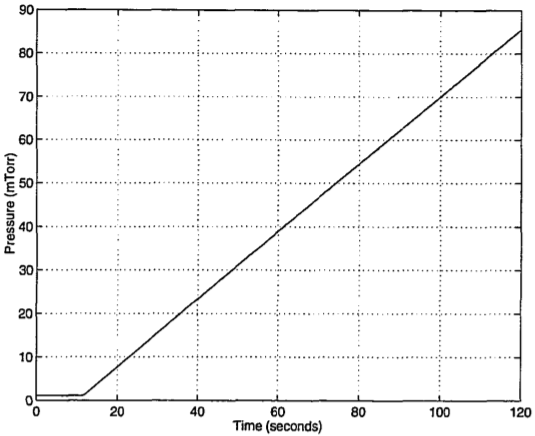
\includegraphics[scale = .75]{Figure 3.5}
	\bf\caption{ Pressure response during volume experiment with a Ar flow of 14 sccm.}
	\label{fig:3.5}
\end{figure}

\setstretch{1.5}
All that remained was to find the volume of the chamber. This was found by isolating the chamber from the pumping stack and measuring the pressure rise at a fix flow rate. The throttle valve could not be used to isolate the chamber, because there is a small (but significant for this experiment) amount of leakage when the valve is fully closed. However, on the AME-8300 there is a turbo gate valve directly above throttle valve; this valve is effective at shutting off flow out of the chamber and was thus used. The throttle valve and the turbo gate valve are very close together, thus using the gate valve does not significantly change the chamber volume. The response of the pressure during this experiment is shown in Figure 3.5.


Prom this data, the pressures $P_{1}$ and $P_{2}$ were recorded at times $t_{1}$ and $t_{2}$, respectively.

From the flow rate ($flw$), the standard volume\footnote{The volume of gas is measured at standard pressure (760 Torr) and temperature (298°K).} of gas added ($V_{added}$) was calculated,

\setstretch{1}
\begin{align}
	V_{added} = flw \times \Delta t
\end{align}

\setstretch{1.5}
\noindent where $\Delta t = t_{2} — t_{1}$. One mole of gas at standard temperature and pressure occupies a volume of $22.4 x 10^{-3}m^{3} [110]$. Next, the number of moles added ($\Delta n$) was computed by


\setstretch{1}
\begin{align}
	\Delta n = \frac{V_{added}}{22.4 x 10^{-3}m^{3}}
\end{align}

\noindent This allowed the volume of the chamber ($V_{cham}$) to be determined by

\begin{align}
	V_{cham} = \frac{\Delta n RT}{\Delta P}
\end{align}

\noindent where $\Delta P = P_{2} — P_{1}$. From this experiment, the chamber volume was calculated to be

\begin{align}
	V_{cham} = 0.211.
\end{align}

\noindent This value was verified by repeating the experiment with different flow rates and gases.

\setstretch{1.5}
Finally, the flow through the throttle valve was calculated using Equation 3.2. Figure 3.6 shows this flow vs. various throttle positions and pressures. From this figure it is seen that the throttle valve has the most authority at settings between 12.5 and 15.0 \%Open. It was determined that for a throttle position of 12.5 \%Open, a $CF_{4}$ flow rate of 30 seem yielded a chamber pressure of 20 mTorr. This operating point was used to develop the model for the plasma generation process and is given again in Table 3.1.

\subsection{Dynamic Model}

\tab The feedback controller design was based on a dynamic model of the plasma generation process. There are several different models that can be used to represent these dynamics. First principle models, such as [64], have the potential of providing a detailed physical


\setstretch{1}
\begin{figure}[H]
	\centering
	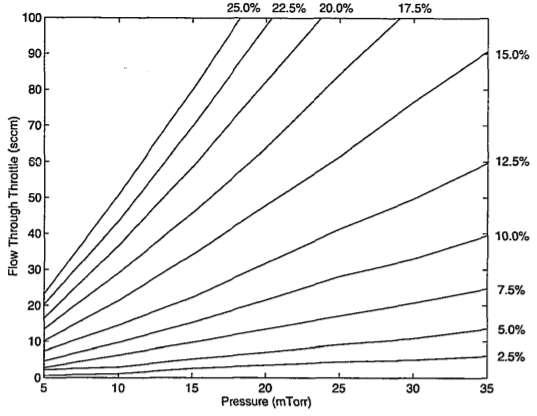
\includegraphics[scale = .75]{Figure 3.6}
	\bf\caption{  Flow through the throttle valve vs. pressure and throttle position.}
	\label{fig:3.6}
\end{figure}

\setstretch{1.5}
\noindent description of the system. Unfortunately, the modeling of plasma and surface reactions is very complex and these models are not well suited for use in real-time feedback control. Another approach is to empirically develop models with input-output data from the system. These models, while easy to develop, only apply to the reactor from which the data was collected. In addition, these models provide little insight into the underlying mechanisms of the process [12]. Many empirical models of plasma etching processes (see, for example, [2,3,57]) only give a static relationship between equipment inputs and etch characteristics. Those used for real-time feedback control need to be dynamic in nature. Between these two extremes are phenomenological models [15]. Phenomenological models attempt to capture only the dominant physical mechanisms and are often empirically tuned to a specific reactor or process.


In this research, 1 have primarily used empirical models of the plasma generation process. The fluorine concentration estimate was based on the physics presented in Section 2.1.3.

\setstretch{1}
\begin{table}[H]
	\centering
	\begin{tabular}{|c|c|}
		\hline
		Throttle Position & 12.5 \%Open \\
		\hline
		$\text{CF}_{4}$ Flow Rate & 30 sccm \\
		\hline
		Applied Power & 1000 W \\
		\hline
	\end{tabular}
	\bf\caption{ Operating point for the plasma generation process model.}
	\label{Table:3.1}
\end{table}

\setstretch{1.5}
However, the estimate itself was empirically related to the inputs of the plasma generation process. The PGP model was based on input-output data collected by separately applying steps to the inputs of our reactor. In the rest of this chapter, 1 present the procedure through which this model was developed.

The initial goal of the control strategy was to use throttle position, $CF_{4}$ flow rate, and power to control the three plasma parameters as shown in Figure 3.2. In order to independently set the steady-state values for all of these properties, the dc gain matrix between the equipment inputs and plasma characteristics must be invertible. This dc gain matrix was found by separately changing each actuator settings allowing the system to settle, and taking the ratio of the change in each plasma property to the change in the input. For the plasma generation process the dc gain matrix had the following form\footnote{The original dc gain matrix upon which conclusions were drawn was not available at the time of writing	of this dissertation. Therefore, presented here is a similar dc gain matrix that was recently collected by Oliver Patterson.}

\setstretch{1}
\begin{align}
	\mbox{\scriptsize$\begin{bmatrix} V_{bias} \\ \text{Pressure} \\ [F]\end{bmatrix} = \begin{bmatrix}	0.330 & -0.254 & 0.740 \\ -1.000 & 1.460 & 0.000 \\ 0.246 & 0.205 & 1.760\end{bmatrix} \begin{bmatrix} \text{Throttle Position} \\ \text{CF}_{4} \text{Flow Rate} \\ \text{Power.}	\end{bmatrix}$}
\end{align}

\setstretch{1.5}
\noindent The invertibility of this matrix is measured by its condition number $\kappa$. The condition number is the ratio of the largest to smallest singular value of the matrix\footnote{For a complete description of singular values and matrix condition numbers see [54].}. The singular values for the dc gain matrix were

\setstretch{1}
\begin{align}
	\sigma = \begin{bmatrix} 1.966 & 1.785 & 0.004626 \end{bmatrix},
\end{align}

\noindent and the condition number was

\begin{align}
	\kappa=425.
\end{align}

\setstretch{1.5}
\noindent This implied that the dc gain matrix was almost singular (noninvertible) and that all three outputs could not be independently controlled. The throttle position and flow inputs are almost redundant; they both primarily affect the plasma through pressure. Of the three outputs, $\text{V}_{bias}$ and fluorine concentration most directly affect the etch characteristics; therefore it was decided to regulate these two plasma properties with the feedback controller. The throttle valve was chosen over the flow controller as a manipulated input to the plasma generation process, because the throttle had a quicker time response and slightly higher command authority. For the remainder of this work, flow rate was held fixed at 30 sccm.

In collecting the data for the step experiments, it was noted that the fluorine concentration measurement was very noisy. One possible method to remove some of this noise is to lower the corner frequency of the lock-in filter; however this could potentially filter out some of the dynamics of the fluorine response. An alternative was to repeat the step experiment several times and average the responses together, thus improving the signal-to-noise ratio while preserving the time response of the signals. The $V_{bias}$ and fluorine concentration responses to the steps in power are shown in Figures 3.7 and 3.8. As can be seen in Figure 3.9, this averaging technique greatly improves the signal-to-noise ratio of the fluorine concentration estimate.

The step response data was then used to determine a model for the plasma generation process. This was done by separately identifying a transfer function for each of the input

\setstretch{1}
\begin{figure}[H]
	\centering
	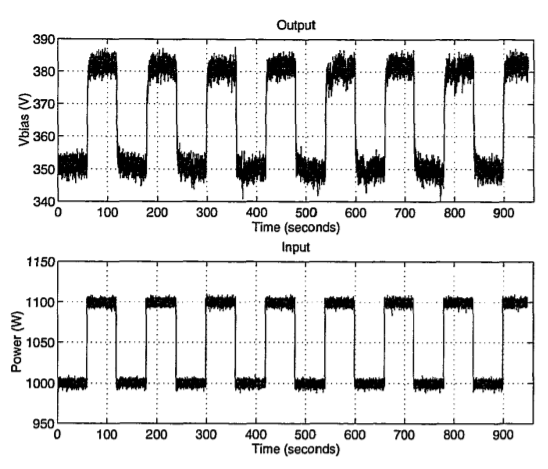
\includegraphics[scale = .7]{Figure 3.7}
	\bf\caption{ $\mathbf{V_{bias}}$ data from power step experiment.}
	\label{fig:3.7}
\end{figure}

\begin{figure}[H]
	\centering
	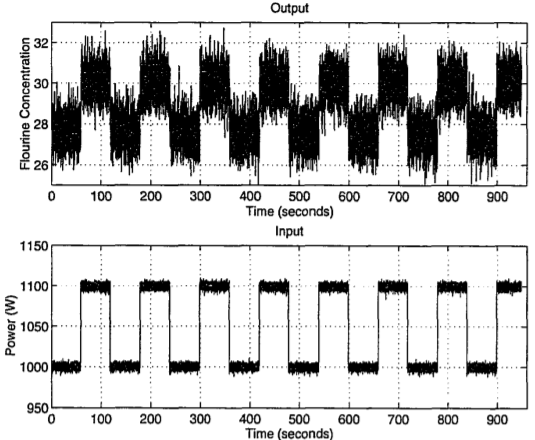
\includegraphics[scale = .7]{Figure 3.8}
	\bf\caption{ Fluorine concentration data power step experiment.}
	\label{fig:3.8}
\end{figure}

\begin{figure}[H]
	\centering
	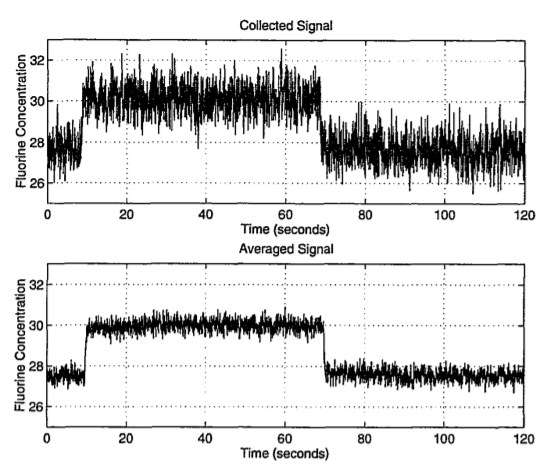
\includegraphics[scale = .7]{Figure 3.9}
	\bf\caption{ Noise reduction due to averaging of [F] signal.}
	\label{fig:3.9}
\end{figure}

\setstretch{1.5}
\noindent output pairs. There are several different linear model structures that can be used to capture the dynamics of a system. A complete description of the various model structures can be
found in [69,98]. Each of these model structures is characterized by a number of parameters which are empirically determined through a least squares optimization; this process is known
as system identification. Initially, several different model structures were compared; the Auto-Regressive Moving Average with eXogenous input (ARMAX) model provided the best fit to the experimental data and was used to model the plasma generation process. In practice, it is often useful to overparameterize the model [69]; this may lead to better fits with the experimental data. The extraneous parameters can later be removed. The system
identification algorithms used in this dissertation generate discrete-time models which were then converted to continuous time for controller design.

\setstretch{1}
\begin{table}[H]
	\centering
	\renewcommand{\arraystretch}{2}
	\begin{tabular}{|c|c|c|c|}
		\hline
		Order & Transfer Function & DC Gain & Mean Square Error \\
		\hline 
		First Order & \large{$\frac{0.3726}{s+1.195}$} & 0.3118 & 0.772 \\
		\hline
		Second Order & \large{$\frac{0.6593(s+7.543)}{(s+1.085)(s+14.639)}$} & 0.3131 & 0.739 \\
		\hline
		Third Order & \large{$\frac{0.4679(s+0.467)(s+1.9828)}{(s+0.362)(s+1.923)(s+1.9832)}$} & 0.3136 & 0.593 \\
		\hline
	\end{tabular}
	\renewcommand{\arraystretch}{1}
	\bf\caption{ Transfer functions from power to $\mathbf{V_{bias}}$ Power to $\mathbf{V_{bias}}$ Response}
	\label{Table:3.2}
\end{table}

\setstretch{1.5}
As can be seen from this Table and the simulated step responses in Figure 3.11, the third order model had the best fit to the experimental data. The differences in the models can be seen from the Bode plots in Figure 3.12. Note that the third order model has an almost pole-zero cancelation; removing the pole-zero pair yields a second order model that fits the experimental data better than the second order model obtained 

\setstretch{1}
\begin{figure}[H]
	\centering
	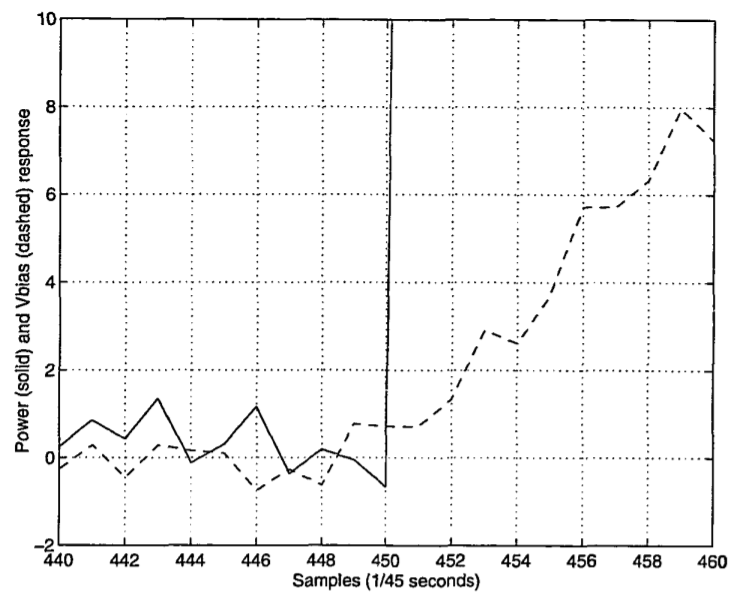
\includegraphics[scale = 0.55]{Figure 3.10}
	\bf\caption{ Delay in response of $\mathbf{V_{bias}}$ to a step in power.}
	\label{fig:3.10}
\end{figure}

\setstretch{1.5}
\noindent directly from the identification. In principle, the second order model obtained directly should be optimal; however, the parameters of this model are obtained by the gradient search technique and thus may have converged only to a local minimum. Therefore, by removing the pole-zero pair for the third order model, the following second order transfer function for the response from power to $V_{bias}$ was found to be


\setstretch{1}
\begin{align}
	G_{vp}(s) = \frac{0.468(s+0.467)}{(s+0.362)(s+1.923)}.
\end{align}

\setstretch{1.5}
\noindent\textbf{Power to Fluorine Concentration Response}

Next, the transfer function for the response from power to estimated fluorine concentration was identified. As with the response of $V_{bias}$ to this input, the fluorine concentration
also responds with a delay of only one sample. This can be seen in Figure 3.13. The armcix command was again used to identify first, second, and third


\setstretch{1}

\begin{figure}[H]
	\centering
	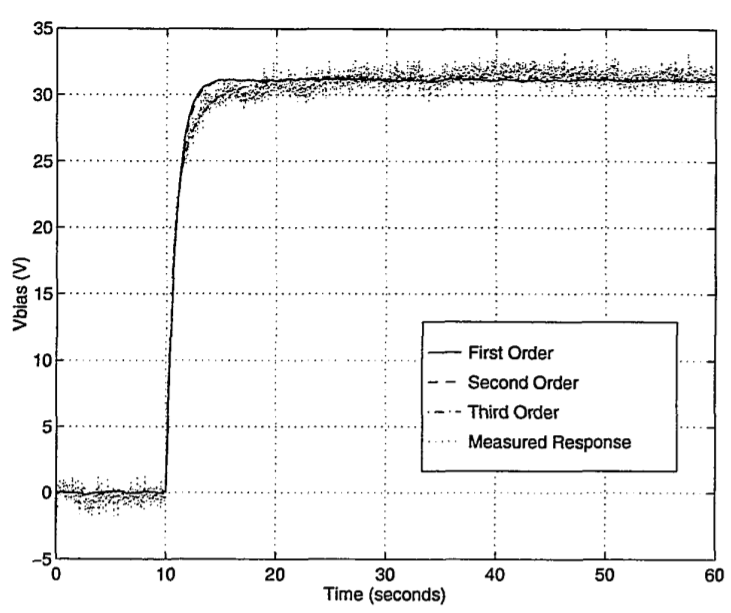
\includegraphics[scale = .55]{Figure 3.11}
	\bf\caption{ Step response: Power to $\mathbf{V_{bf}}$.}
	\label{fig:3.11}
\end{figure}

\begin{figure}[H]
	\centering
	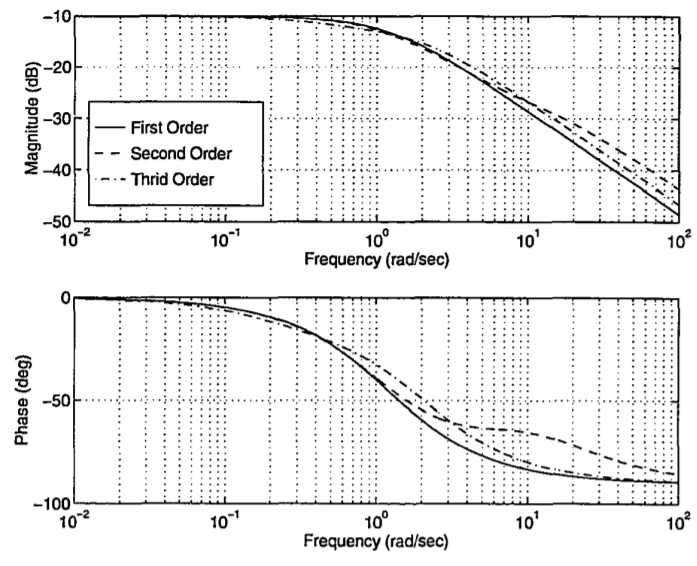
\includegraphics[scale = .55]{Figure 3.12}
	\bf\caption{ Bode plot: Power to $\mathbf{V_{bias}}$.}
	\label{fig:3.12}
\end{figure}

\begin{figure}[H]
	\centering
	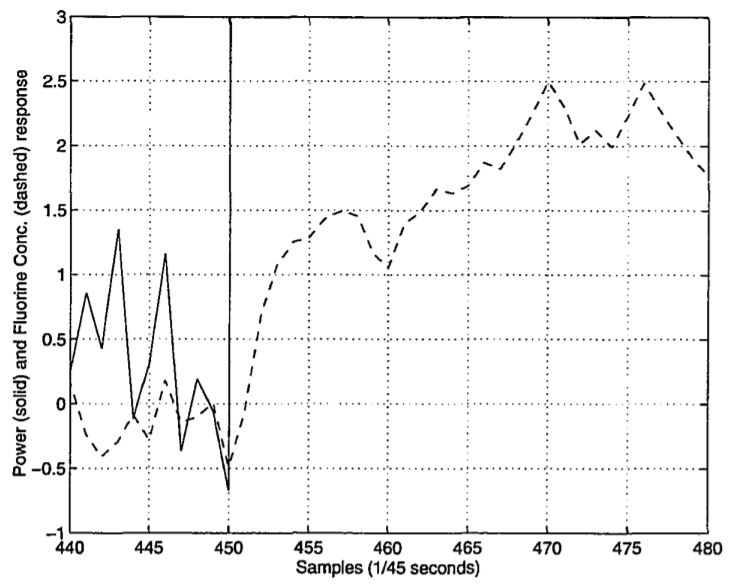
\includegraphics[scale = .55]{Figure 3.13}
	\bf\caption{  Delay in response of fluorine concentration to a step in power.}
	\label{fig:3.13}
\end{figure}

\begin{table}[H]
	\centering
	\renewcommand{\arraystretch}{2}
	\begin{tabular}{|c|c|c|c|}
		\hline
		Order & Transfer Function & DC Gain & Mean Square Error \\
		\hline 
		First Order & \large{$\frac{0.4314}{s+27.61}$} & 0.0245 & 0.248 \\
		\hline
		Second Order & \large{$\frac{0.4598(s+6.275)}{(s+2.662)(s+44.07)}$} & 0.0246 & 0.230 \\
		\hline
		Third Order & \large{$\frac{0.5630(s+5.54)(s+34.47)}{(s+2.48)(s+36.29)(s+48.23)}$} & 0.0246 & 0.230 \\
		\hline
	\end{tabular}
	\renewcommand{\arraystretch}{1}
	\bf\caption{ Transfer functions from power to fluorine concentration.}
	\label{Table:3.3}
\end{table}

\setstretch{1.5}
\noindent  order models; these are given in Table 3.3. A comparison of the step responses of each of these models, seen in Figure 3.14, shows that both the second and third order transfer functions do an adequate job of fitting the measured response. Indeed, as shown in Figure 3.15, the Bode plots of these models are very similar. This is a result of a near pole-zero cancelation in the third order model. It was concluded that that was an adequate representation of the response fluorine concentration to a step in power. Though the pole at -44.07 has no significant effect on the response, it is retained to keep
the transfer function strictly proper. This simplifies the controller design by providing a model with no direct feedthrough term.

\setstretch{1}
\begin{align}
	G_{vp}(s) = \frac{0.460(s+6.28)}{(s+2.66)(s+44.07)}.
\end{align}

\begin{figure}[H]
	\centering
	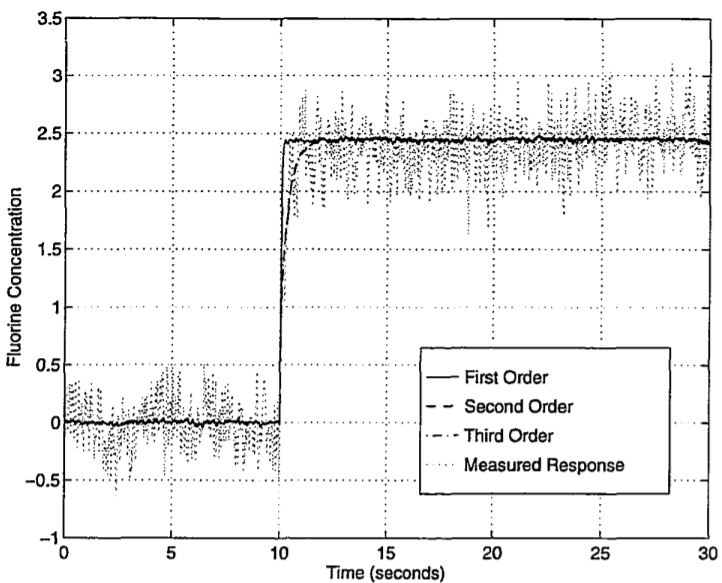
\includegraphics[scale = .55]{Figure 3.14}
	\bf\caption{  Step response: Power to fluorine concentration.}
	\label{fig:3.14}
\end{figure}

\setstretch{1.5}

\noindent \textbf{Throttle Position to $\mathbf{V_{bias}}$ Response}

The response of the system to a step change in throttle position was identified next. Determining the pure time delay for this response was more difficult than in the previous cases. There was a gradual initiation in the response and this coupled with noise made it difficult determine the time delay. Therefore to assist in calculating this delay, a line was drawn tangent to the rising slope of the response and extended back through the x-axis, as shown in Figure 3.16. From a close-up view of the region where this line intercepts the axis (Figure 3.17), the delay was determined to be approximately 28 samples or 0.622 seconds.

\setstretch{.75}
\begin{figure}[H]
	\centering
	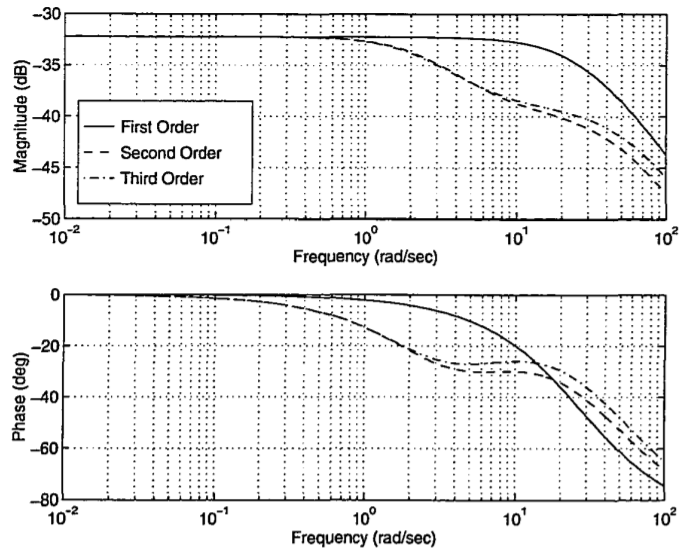
\includegraphics[scale = .5]{Figure 3.15}
	\bf\caption{  Bode plot: Power to fluorine concentration.}
	\label{fig:3.15}
\end{figure}

\begin{table}[H]
	\centering
	\renewcommand{\arraystretch}{2}
	\begin{tabular}{|c|c|c|c|}
		\hline
		Order & Transfer Function & DC Gain & Mean Square Error \\
		\hline 
		First Order & \large{$\frac{2.80}{s+0.174}$} & 16.08 & 0.614 \\
		\hline
		Second Order & \large{$\frac{2.98(s+3.48)}{(s+0.173)(s+3.72)}$} & 16.08 & 0.618 \\
		\hline
		Third Order & \large{$\frac{-0.768(s+2.35)(s-68.46)}{(s+0.175)(s+2.58)(s+16.30)}$} & 16.10 & 0.611 \\
		\hline
	\end{tabular}
	\renewcommand{\arraystretch}{1}
	\bf\caption{ Transfer functions from throttle position to $\mathbf{V_{bias}}$}
	\label{Table:3.4}
\end{table}

\setstretch{1.5}
The various order identified models are shown in Table 3.4. The dominant pole in each of these models was around s = —0.174. Indeed both the step responses (Figure 3.18 and Bode plots 3.19 show similar responses for all of these models. Thus, for this input-output pair the transfer function model was found to be

\setstretch{1}
\begin{align}
	G_{vt}(s)=\frac{2.80e^{-0.622\tau}}{s+0.174},
\end{align}

\noindent where $e^{-0.622\tau}$ represents the time delay of $\frac{28}{45}$ seconds.

\setstretch{1}
\begin{figure}[H]
	\centering
	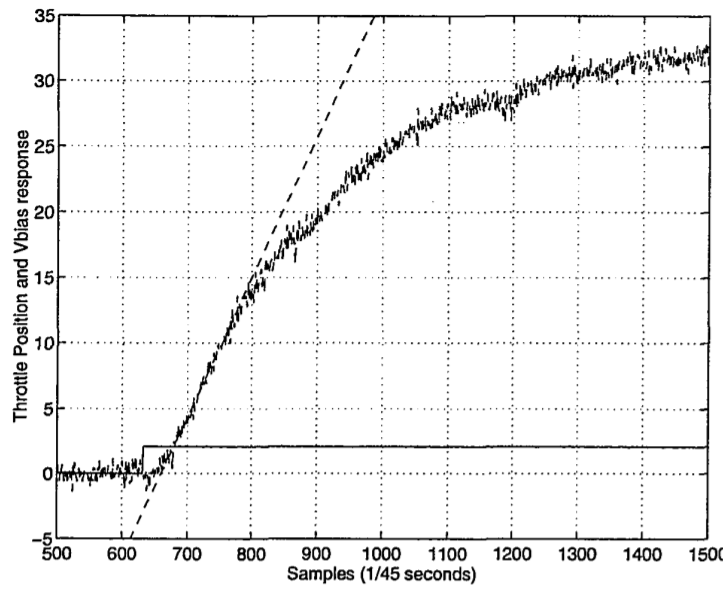
\includegraphics[scale = .5]{Figure 3.16}
	\bf\caption{  Delay in response of $\mathbf{V_{bias}}$ to a step in throttle position.}
	\label{fig:3.16}
\end{figure}

\begin{figure}[H]
	\centering
	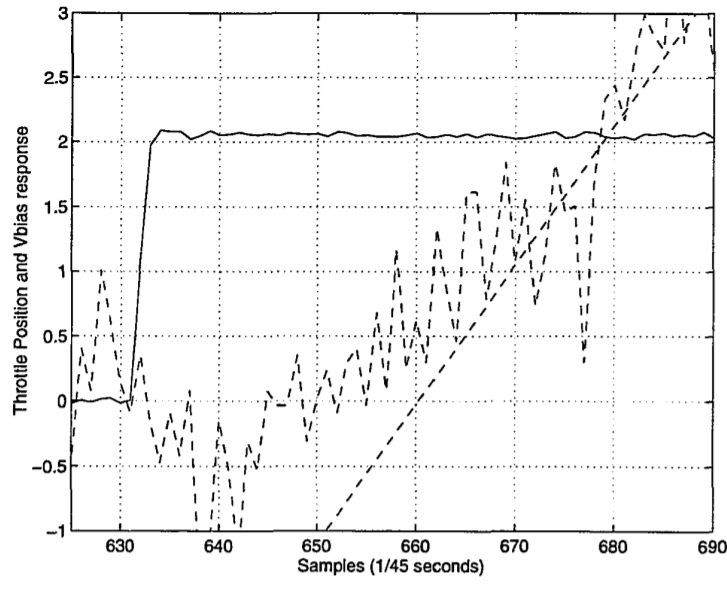
\includegraphics[scale = .5]{Figure 3.17}
	\bf\caption{  Detailed view of the delay in response of $\mathbf{V_{bias}}$ to a step throttle position.}
	\label{fig:3.17}
\end{figure}

\begin{figure}[H]
	\centering
	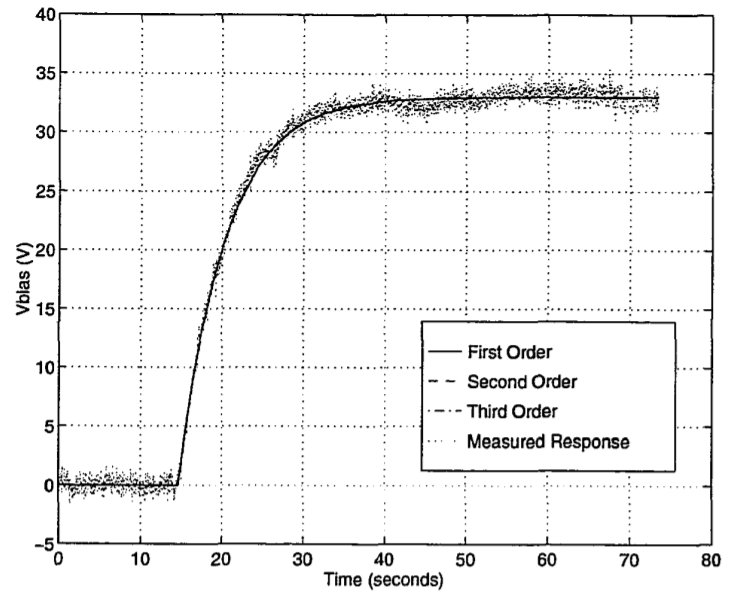
\includegraphics[scale = .5]{Figure 3.18}
	\bf\caption{  Time response: Throttle position to $\mathbf{V_{bias}}$.}
	\label{fig:3.18}
\end{figure}

\begin{figure}[H]
	\centering
	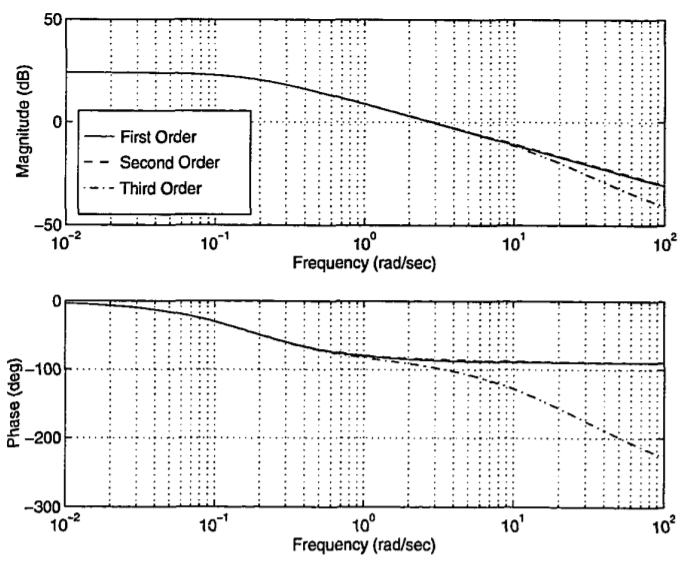
\includegraphics[scale = .5]{Figure 3.19}
	\bf\caption{  Bode plot: Throttle position to $\mathbf{V_{bias}}$.}
	\label{fig:3.19}
\end{figure}

\begin{figure}[H]
	\centering
	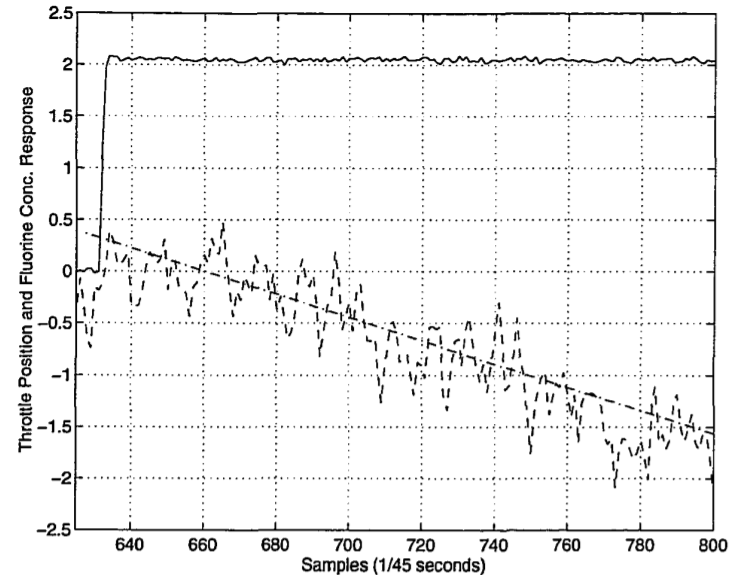
\includegraphics[scale = .5]{Figure 3.20}
	\bf\caption{  Delay in response of fluorine concentration to a step in throttle position. }
	\label{fig:3.20}
\end{figure}

\setstretch{1.5}
\noindent \textbf{Throttle Position to Fluorine Concentration Response}

The final transfer function to be identified was for the response of fluorine concentration to a step in throttle position. The time delay was determined in the same manner as the one for the $V_{bias}$ response. As is shown in Figures 3.20 and 3.21, the delay is again approximately 28 samples. The identified transfer functions are shown in Table 3.5. In this case, the second and third order models accurately simulate 

\setstretch{1}
\begin{table}[H]
	\centering
	\renewcommand{\arraystretch}{2}
	\begin{tabular}{|c|c|c|c|}
		\hline
		Order & Transfer Function & DC Gain & Mean Square Error \\
		\hline 
		First Order & \large{$\frac{-3.98}{s+2.03}$} & -1.93 & 0.728 \\
		\hline
		Second Order & \large{$\frac{4.03(s-3.56)}{(s+0.204)(s+33.38)}$} & -2.10 & 0.300 \\
		\hline
		Third Order & \large{$\frac{3.91(s+2.42)(s-3.61)}{(s+0.204)(s+2.39)(s+33.33)}$} & -2.10 & 0.300 \\
		\hline
	\end{tabular}
	\renewcommand{\arraystretch}{1}
	\bf\caption{ Transfer functions from throttle position to fluorine concentration.}
	\label{Table:3.5}
\end{table}

\begin{figure}[H]
	\centering
	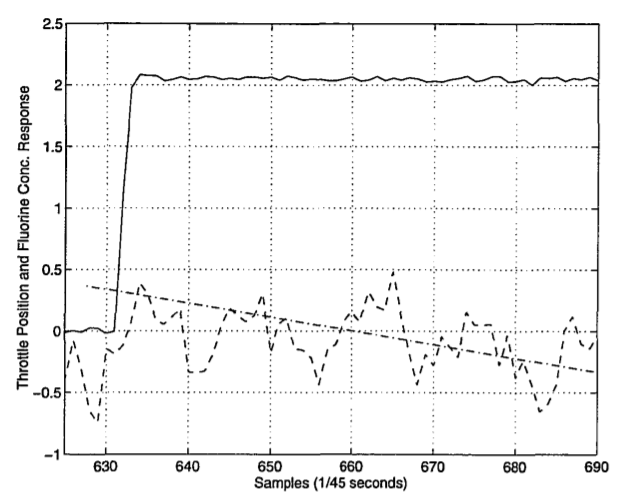
\includegraphics[scale = .5]{Figure 3.21}
	\bf\caption{  Detailed view delay in response of fluorine concentration to a step in throttle position.}
	\label{fig:3.21}
\end{figure}

\setstretch{1.5}
\noindent the fluorine response. This is shown in Figure 3.23. Likewise, both of these models have similar Bode plots (Figure 3.22).
In each model, the pole at $s = —0.204$ dominates the other poles and zeros. Therefore, including the time delay, the model was reduced to


\setstretch{1}
\begin{align}
	G_{Ft}(s) = \frac{-0.428e^{-0.622\tau}}{s+0.204}
\end{align}

\setstretch{1.5}

\noindent\textbf{Full Model}

The full system was modeled by combining the four individual transfer function (Equations 3.12, 3.13, 3.14, and 3.15) into a 2 x 2 transfer function matrix.

\setstretch{1}
\begin{figure}[H]
	\centering
	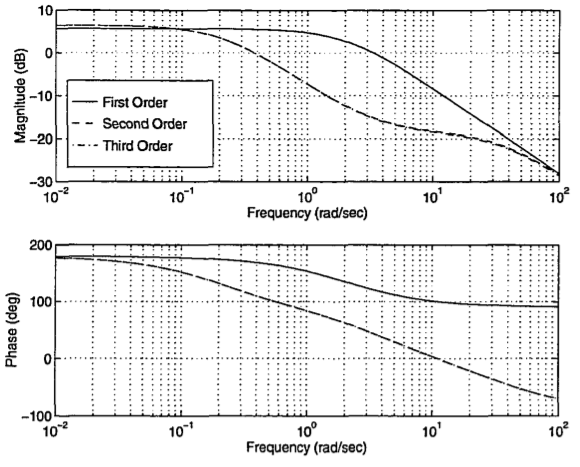
\includegraphics[scale = .6]{Figure 3.22}
	\bf\caption{  Bode plot: Throttle position to fluorine concentration.}
	\label{fig:3.22}
\end{figure}

\begin{figure}[H]
	\centering
	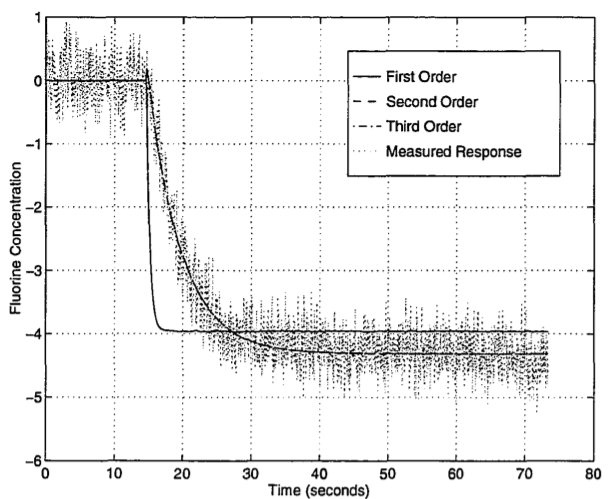
\includegraphics[scale = .6]{Figure 3.23}
	\bf\caption{  Time response: Throttle position to fluorine concentration.}
	\label{fig:3.23}
\end{figure}

\begin{align}
	\renewcommand\arraystretch{2} \begin{bmatrix} V_{bias} \\ [F] \end{bmatrix} = \begin{bmatrix} \frac{2.80e^{-0.622\tau}}{s+0.174} & \frac{0.468(s+0.467)}{(s+0.362)(s+1.923)} \\ \frac{-0.428e^{-0.622\tau}}{s+0.204} & \frac{0.460(s+6.28)}{(s+2.66)(s+44.07)}  \end{bmatrix} \begin{bmatrix} \text{Throttle Position} \\ \text{Power} \end{bmatrix}
\end{align}

\setstretch{1.5}

\section{Model Validation}

\tab In order to determine if the 2 x 2 transfer function model was a good approximation of the physical system, an experimental test was performed. The model was identified by exciting the system with only one actuator at a time; in the real system, it is of course possible to vary both the throttle position and power simultaneously. In principle, our linear model should predict the response to small simultaneous variations in the actuators with the same fidelity as it predicts the response to individual variations. In practice, however, the model may fail to accurately describe the system response due to neglected nonlinearities. To test the fidelity of our model’s ability to describe simultaneous actuator variations, two simultaneous pseudo random binary signals (PRBS) [98] were applied to the actuators; these are shown in Figure 3.24. The PRBS applied to the throttle position was given a slower switching rate because the dynamics associated with the throttle were slower than those associated with the power input. The response of the model and the actual system, as well as the error between them, is plotted in Figure 3.25 for the $V_{bias}$ signal. As can be seen from this plot, except for a small bias in the response, the model accurately represents the dynamics of the system; a tentative explanation for this bias is that it is due to nonlinearity. A similar comparison for fluorine concentration is shown in Figure 3.26. In this case the resulting error shows very little bias, though the signal-to-noise ratio is very poor.

\setstretch{1}
\begin{figure}[H]
	\centering
	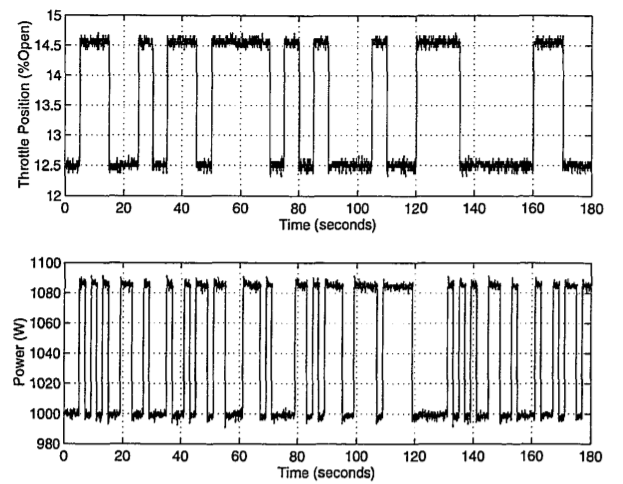
\includegraphics[scale = .6]{Figure 3.24}
	\bf\caption{ PRBS applied in model validation experiment.}
	\label{fig:3.24}
\end{figure}

\begin{figure}[H]
	\centering
	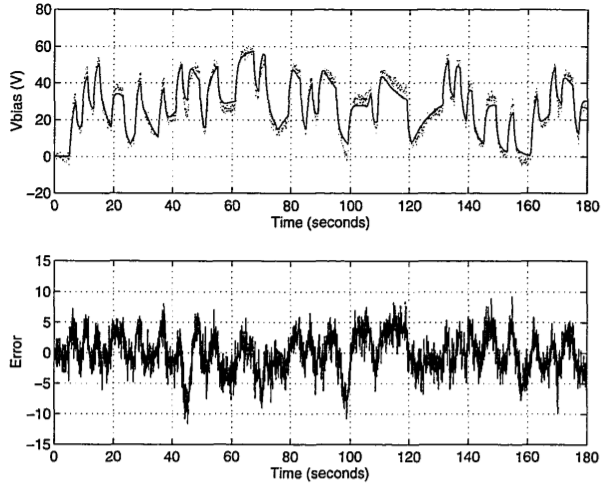
\includegraphics[scale = .6]{Figure 3.25}
	\bf\caption{  Comparison of actual and simulated $\text{V}_{bias}$ response to simultaneous PRBS inputs.}
	\label{fig:3.25}
\end{figure}

\begin{figure}[H]
	\centering
	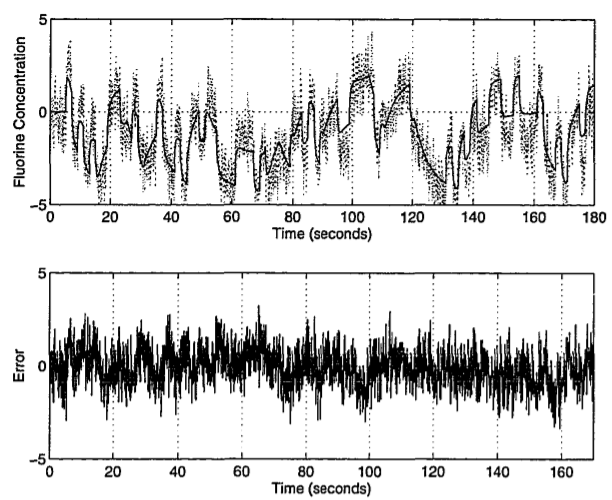
\includegraphics[scale = .75]{Figure 3.26}
	\bf\caption{ Comparison of actual and simulated fluorine concentration response to simultaneous PRBS inputs.}
	\label{fig:3.26}
\end{figure}